In the following, we focus on operational semantics of models that are defined by a set of graph transformation rules.
In \cref{fig:sec-compl-oper-sem:oper}, two rules are presented that define aspects of the operational semantics of UML statecharts from \cref{sec-gen-intro-models}.
Rule \code{S2S-Simple} defines the \code{Transition} from on \code{State} to another state in the statechart but only if the transition performs no \code{action} when being fired as ensured by the negative application condition (NAC).
When being applied, the rule moves the \code{Token} from the source (\code{src}) state of the transition to the target (\code{tgt}) state by deleting the active token and creating a new token and assigned it to the target state.
Similarly, we define rule \code{S2S-Action} that performs a transition from a source to a target state if the transition performs an action when being fired.
Simultaneously, the rule fires the transition with that event which is in correspondence with the action.

Therefore, both rules define a token semantics by replacing tokens.
The deleted token points to the source part of the graph (marked with \code{S}) and the created token points to the target part of the graph (marked with \code{T}).
We can intepret both rules as non-deleting rules where the \code{S} has to exist and the \code{T} part is being created by the rule.
Therefore, we can apply the verification of domain completeness in order to verify if all elements in UML statecharts are covered by the operational semantics.
As the verification is restricted to graph grammars with empty start graphs only, an additional rule has to be defined which creates the initial token to the initial state of the statechart.
The verification returns minimal examples of statechart excerpts that cannot be completely covered by the semantics.
This can be taken as the basis for the definition of a set of domain constraints that successively restrict the structure of statecharts such that they can be completely simulated.
The constraints may serve as guidelines for modellers, e.g., in order to avoid statecharts with deadlocks.
Note that in the case of statecharts, the constraints will only allow to represent single processes without choices in the statechart.
However, single traces can simply be combined to more complex statecharts with choices.

\begin{figure}[!tb]
\begin{center}
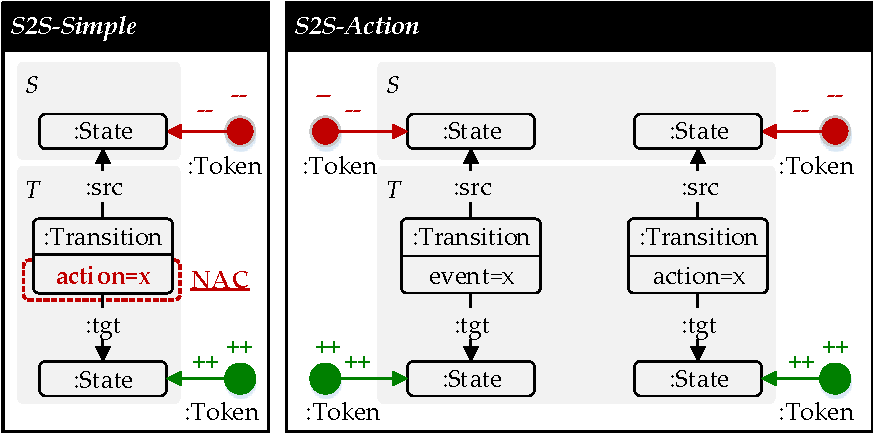
\includegraphics[width=.7\textwidth]{img/semantics/dynamic.pdf}
\end{center}
\caption{Operational Semantics of UML Statecharts}
\label{fig:sec-compl-oper-sem:oper}
\end{figure}
